En esta sección se presentan algunos de los fundamentos teóricos acerca de las tecnologías de virtualización, los cuales permiten brindar claridad en la terminología para establecer una base común de contextualización utilizado en el presente trabajo.  El marco conceptual comprende secciones relacionadas con los \textit{fundamentos}, \textit{contexto histórico} y los \textit{ámbitos de aplicación} de las tecnologías de vitualización, los cuales se describen a continuación.

% Sección: Fundamentos de la virtualización
\section{Fundamentos de la virtualización}\label{fundamentos}

Para realizar una referencia a los fundamentos teóricos, a continuación, se presentan en primera instancia el concepto mismo de la virtualización, seguido de elementos y técnicas de utilización; además se presenta la  taxonomía de referencias utilizada en el presente trabajo. 

\subsection{Virtualización}

La virtualización puede ser considerada como la combinación de diferentes tecnologías, que ofrece a las organizaciones gran variedad de ventajas como el apoyo para la gestión de grandes volúmenes de datos, la posibilidad de escalar rápidamente la infraestructura de aplicaciones y el aprovechamiento de grandes capacidades de cómputo; técnicamente y según lo señala \textcite{Kusnetzky2011}, la virtualización permite abstraer aplicaciones y los componentes subyacentes de hardware para ser presentados como una vista lógica o virtual de estos recursos \parencite{AbdElRahem2016}. Esta vista lógica puede ser en ocasiones notablemente diferente a la vista física, la cual por lo general se construye a partir del exceso de recursos de computación, tales como el poder de  procesamiento, la memoria, la capacidad de almacenamiento o incluso el ancho de banda \parencite{Stallings2015}.\\

En complemento a lo anterior, \textcite{Silberschatz2014} señalan que la virtualización está relacionada con la tecnología que permite que los sistemas operativos se ejecuten como aplicaciones dentro de otros sistemas operativos. \\

La virtualización también incluye el término \textit{emulación}, el cual es ampliamente conocido y hace referencia al hecho de tener diferencias entre la arquitectura base y la proyectada en el proceso de virtualización.\\

Entre los objetivos de la virtualización se tiene: aumento de los niveles de rendimiento computacional, favorecer la escalabilidad y disponibilidad de sus soluciones tecnológicas de manera eficiente y eficaz, además de propender por unificar y usar de forma fácil las estructuras de administración y seguridad de la infraestructura computacional existente \parencite{Kusnetzky2011, Hui2014}. \\

A través de la virtualización es posible crear una vista lógica  que combine recursos computacionales para presentar uno o varios entornos operativos, esto es por ejemplo, que muchos computadores físicos sean vistos como un único gran recurso (agregación de recursos) o por el contrario, que un solo computador sea visto como múltiples instancias de sí mismo (división de recursos)  \parencite{Silberschatz2014}. La virtualización puede tener lugar usando metodologías como partición o agregación de hardware y software, simulación de máquina parcial o completa, emulación y tiempo compartido entre otros \parencite{Chiueh2005, Hoopes2009}. La partición de recursos es una de las formas más comunes de usar la virtualización, en este caso, es posible agregar la capa de virtualización sobre el recurso real, tal como se muestra en la figura \ref{fig:divisionDeRecursosConVirtualizacion}. Esta capa de virtualización permite que varios recursos virtuales sean ejecutados simultáneamente ubicados sobre un mismo recurso real.

\begin{figure}[!hbtp]
	\centering
	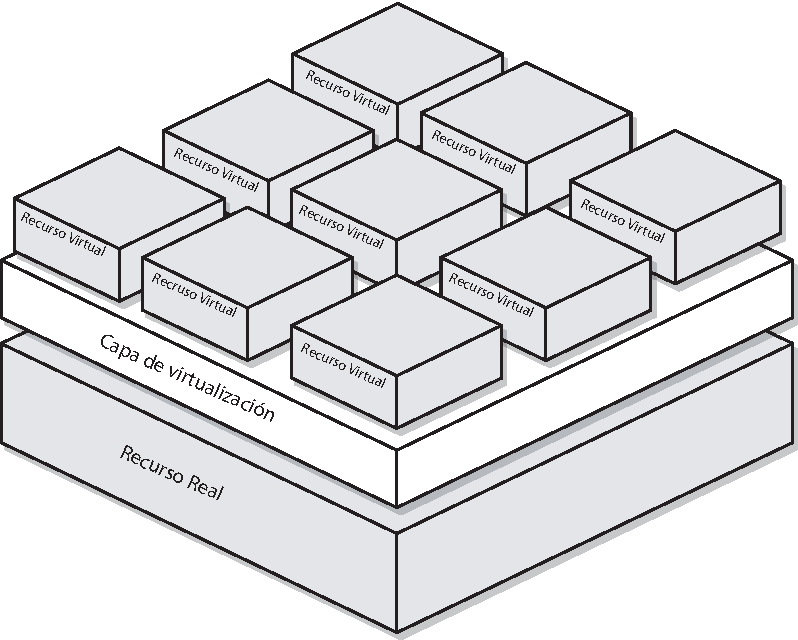
\includegraphics[width=8cm]{Pictures/divisionRecursosFisicosConV12N.pdf}
	\vspace{-0.2cm}
	\caption{División de recursos a través de la virtualización}
	\label{fig:divisionDeRecursosConVirtualizacion}
\end{figure}

Desafortunadamente la arquitectura de computadores x86 a pesar de ser una de las más populares en el mundo, no es virtualizable al 100\% \parencite{Adams}. En esta arquitectura, al ejecutar instrucciones en modo no privilegiado, algunas de ellas pueden fallar silenciosamente en lugar de provocar una trampa y así brindar su respectivo tratamiento. Esta situación ha tenido respuesta a través de mecanismos y formas de virtualización que actúan en diversos niveles de abstracción. Los niveles de abstracción dónde la virtualización tiene lugar son los siguientes: nivel del conjunto de instrucciones, nivel de abstracción de hardware, nivel de sistema operativo, nivel de interfaz de biblioteca de nivel de usuario y finalmente en el nivel de aplicación \parencite{Chiueh2005}.\\

Los conceptos acerca de la virtualización se presentan agrupados en las categorías \textit{elementos} y  \textit{técnicas de la virtualización}, cuya descripción se muestra en los apartados siguientes.


\subsection{Elementos de la virtualización}

Los elementos \textit{máquina real}, \textit{máquina virtual} y \textit{monitor de máquinas virtuales}, son considerados básicos para la comprensión de las tecnologías de virtualización y se describen a continuación.

\subsubsection{Máquina real}

El término \textit{máquina real} (RM por sus siglas en inglés \textit{Real Machine}) referencia los elementos físicos de la infraestructura tecnológica que conforman un computador; ya sea un computador personal, una estación de trabajo o un servidor. Otras referencias a este concepto son los términos en inglés \textit{hardware}, \textit{physical hardware}, \textit{bare-metal}. En el ámbito informático comercial es común que se refiera al concepto de RM utilizando la palabra \textit{anfitrión} o en inglés \textit{host} \parencite{VMware2008}. 

\subsubsection{Máquina virtual}

El concepto de \textit{máquina virtual} (VM por sus siglas en inglés \textit{Virtual Machine}) no es nuevo y fue formalizado en la tesis de  \textcite{Goldberg1973} y publicado en el trabajo académico de \textcite{Goldberg1974}; en estos trabajos se establecen las bases conceptuales para determinar el significado de una VM, siendo esta asumida como un duplicado eficiente y aislado de una RM, ver figura \ref{fig:TheVirtualMachineMonitor_Popek1974}.\\

Actualmente el concepto de VM hace referencia a un ambiente operativo para el conjunto de aplicaciones del nivel de usuario, lo cual incluye librerías, llamados al sistema, interfaces/servicios, configuraciones del sistema, procesos y archivos de estado \parencite{Chiueh2005}. Otra forma de presentar el concepto de VM según \textcite{Solis2014}, es relacionarlo con una capa de software, la cual se posiciona entre los recursos hardware o software y las aplicaciones. También es muy común que en el ámbito informático comercial se refiera al concepto de VM utilizando la palabra \textit{invitado(a)} o en inglés \textit{guest} \parencite{VMware2008}. Finalmente, \textcite{Pek2013} establecen que una VM, es también considerada como una abstracción de recursos de computación presentados como servicio para permitir que éstos operen simultáneamente sobre la misma infraestructura de la RM .

\begin{figure}[!hbtp]
	\centering
	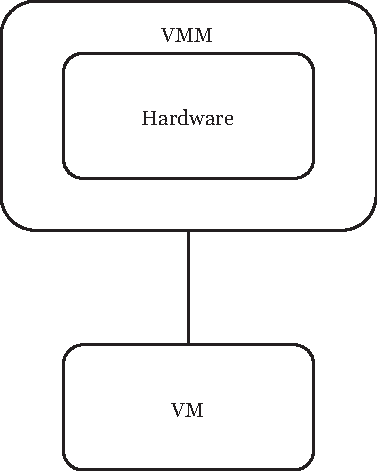
\includegraphics[width=5cm]{Pictures/VMMPopek1974.pdf}
	\vspace{-0.2cm}
	\caption{Visión general de MV y VMM por \textit{Popek} y \textit{Goldberg}.\footnotemark[2]{} }
	\label{fig:TheVirtualMachineMonitor_Popek1974}
\end{figure}

\footnotetext[2]{Basada en la figura original del monitor de máquina virtual del trabajo \textit{formal Requirements for Virtualizable Thrid Generation Architectures} de Gerald J. Popek y Robert P. Goldberg en 1974.}

\subsubsection{Monitor de máquinas virtuales}

El término monitor de máquina virtual (VMM por sus siglas en inglés \textit{Virtual Machine Monitor}), fue establecido en el trabajo de \textit{Popek} y \textit{Goldger} \cite{Popek1974}, en el cual  se definieron las bases conceptuales de un VMM como una pieza de software que tiene las siguientes tres características esenciales: 
\begin{enumerate}
	\item \textit{Equivalencia}: Proveer un ambiente para los programas, el cual es idéntico a la máquina original.\\
	
	\item \textit{Desempeño}: Los programas que se ejecutan en este ambiente muestran, en el peor de los casos, solo una degradación en velocidad.\\
	
	\item \textit{Control de recursos}: El VMM está en completo control de los recursos del sistema.\\ 
\end{enumerate}

La definición de un VMM está relacionada con una capa software que proporciona  infraestructura de soporte utilizando los recursos de un nivel más bajo (generalmente \textit{hardware}), para crear múltiples máquinas virtuales que son independientes y aisladas entre sí \parencite{Chiueh2005, Cafaro2011}. De manera similar, \textcite{Stallings2015}  determina  que un VMM, es un software que actúa como un intermediador entre la RM y las VMs; este software es comúnmente llamado \textit{hipervisor}, el cual permite que muchas máquinas virtuales coexistan de forma segura en una única RM. La cantidad de máquinas virtuales que existen en una sola máquina real, determina el índice de consolidación que para el caso particular de la figura \ref{fig:VMM}, es de 9 a 1 expresado como (9:1). Entre mayor sea el índice de consolidación mejor será el ROI y menos el TCO de la máquina real utilizada. Algunas de las funciones y responsabilidades de los hipervisores son la emulación, aislamiento, asignación de recursos y el encapsulamiento \parencite{Hoopes2009}.

\begin{figure}[!hbtp]
	\centering
	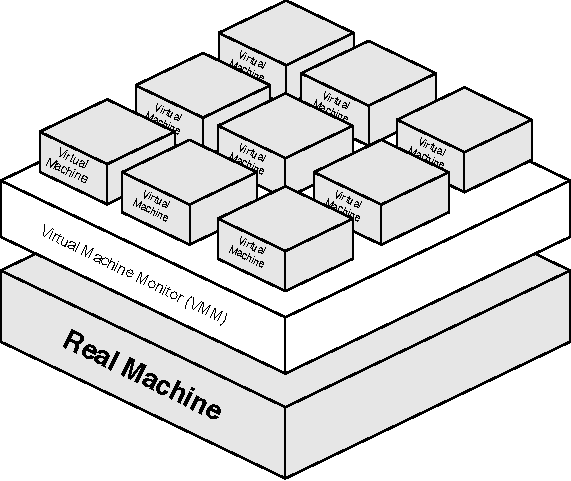
\includegraphics[width=8cm]{Pictures/VMMGeneric.pdf}
	\vspace{-0.2cm}
	\caption{Monitor de máquinas virtuales (VMM) o hipervisor}
	\label{fig:VMM}
\end{figure}

\subsection{Técnicas de virtualización}

A continuación, se describen dos de las principales técnicas de virtualización comúnmente utilizadas con son la \textit{basada en hipersivor} y la \textit{basada en contenedores}, estas técnicas permiten en general lograr consolidar componentes hardware y brindar un ambiente de ejecución virtual para sistemas o procesos respectivamente.

\subsubsection{Virtualización basada en hipervisor}

La técnica de virtualización basada en hipervisor consiste en la utilización del VMM como elemento central, el cual puede estar ubicado de dos maneras diferentes. La primera forma consiste en ubicar el hipervisor directamente sobre el hardware. Esta técnica es también conocida como virtualización \textit{bare-metal} o \textit{nativa}, y al hipervisor se le denomina de \textit{Tipo 1} (Figura \ref{fig:Bare-metalHypervisor}).  La utilización de este tipo de hipervisor no necesita la presencia de un sistema operativo subyacente en la RM. La segunda realiza la instalación del hipervisor sobre un sistema operativo existente. Esta técnica es también conocida como virtualización \textit{alojada} o \textit{basada en host}, y al hipervisor se le considera de \textit{Tipo 2} (ver figura \ref{fig:host-basedHypervisor}). Como característica general de la virtualización basada en hipervisor, se tiene la creación de máquinas virtuales completas, las cuales pueden ejecutar sistemas operativos \textit{guest} independientes y posiblemente diferentes, siempre y cuando sean compatibles con arquitectura virtual entregada. 


\begin{figure}[!hbtp]
	\centering
	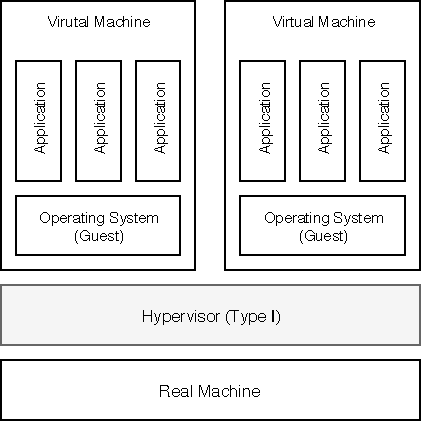
\includegraphics[width=8cm]{Pictures/bare-metalHypervisor.pdf}
	\vspace{-0.2cm}
	\caption{Bare-metal Hypervisor}
	\label{fig:Bare-metalHypervisor}
\end{figure}

\begin{figure}[ht] %[!hbtp]
	\centering
	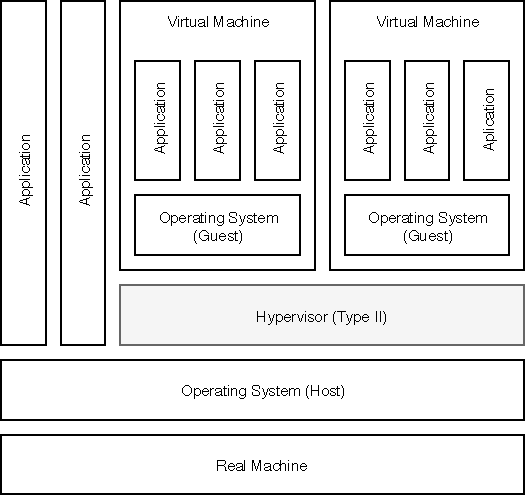
\includegraphics[width=8cm]{Pictures/host-basedHypervisor.pdf}
	\vspace{-0.2cm}
	\caption{Hoste based hypervisor}
	\label{fig:host-basedHypervisor}
\end{figure}

\subsubsection{Virtualización basada en contenedores}

La técnica de virtualización basada en contenedores utiliza como base un sistema operativo preexistente y consiste en la generación de entornos virtuales de ejecución para procesos. Estos entornos de ejecución son comúnmente llamados \textit{contenedores} (ver figura \ref{fig:container-baseVirtualization}). Esta técnica de virtualización gana cada día mayor aceptación en los ámbitos académico y productivo, debido a que, a diferencia de la virtualización basada en hipervisor, no es necesario generar VMs con sistemas operativos completos, sino que se utilizan partes fundamentales del sistema operativo \textit{host} para generar los entornos virtuales de operación para los procesos \parencite{Kon2017}. Lo anterior supone una menor carga computacional necesaria para generar el entorno virtual y de igual forma supone que dicho entorno está sujeto al tipo de sistema operativo subyacente. 


\begin{figure}[ht] % [!hbtp]
	\centering
	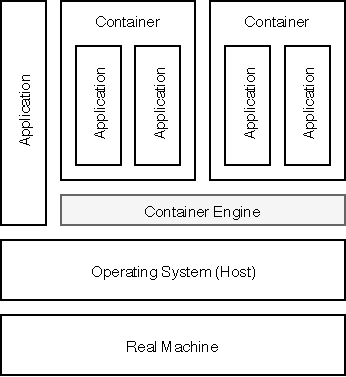
\includegraphics[width=8cm]{Pictures/container-baseVirtualization.pdf}
	\vspace{-0.2cm}
	\caption{Container-based virtualization}
	\label{fig:container-baseVirtualization}
\end{figure}


\subsection{Taxonomía de Tecnologías de Virtualización}



\begin{figure}[!htp]
	\centering
	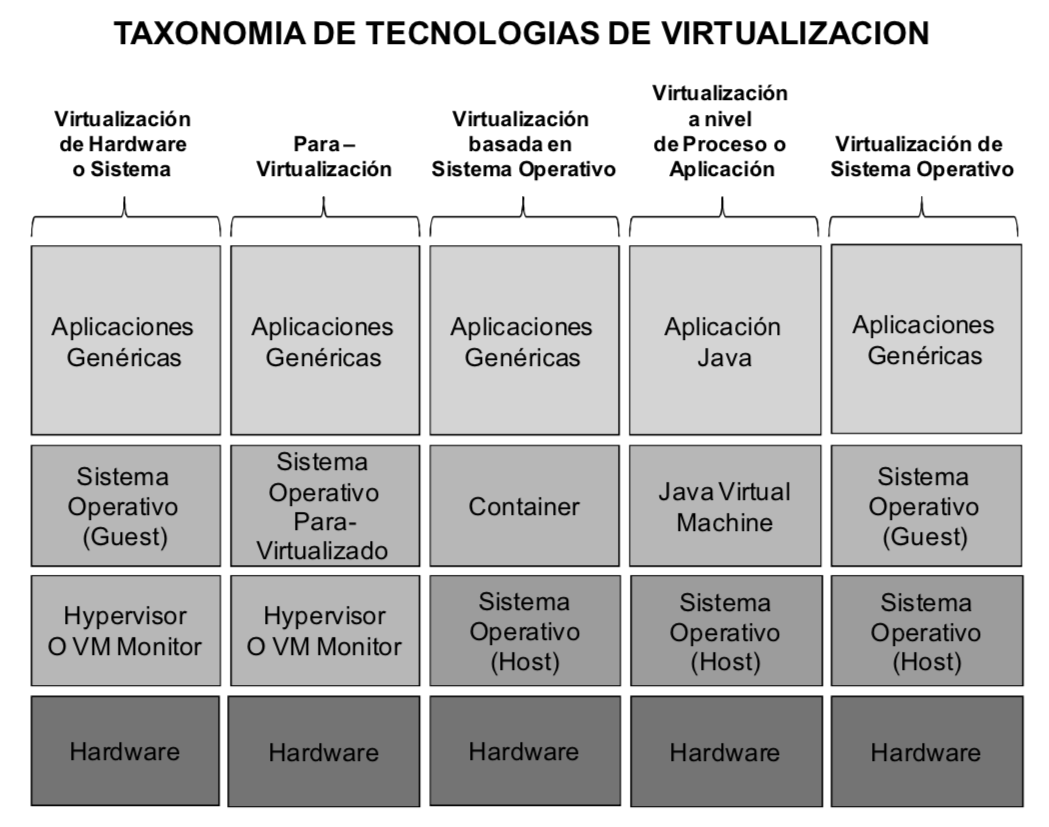
\includegraphics[width=0.8 \linewidth]{Pictures/taxonomiaPessolani.png}
	\vspace{-0.2cm}
	\caption{Taxonomía de máquinas virtuales propuesta por Pessolani y otros en 2012\footnotemark[8]{}}
	\label{fig:taxonomiaPessolani}
\end{figure}

\footnotetext[8]{Figura basada en el trabajo \textit{Sistema de virtualización con recursos distribuidos } de Pablo Pessolani, Toni Cortes, Silvio Gonnet y Fernando Tinetti, en 2005.}

El presente trabajo utiliza como base conceptual la taxonomía de tecnologías de virtualización propuesta por \textcite{Pessolani2012}. Esta taxonomía posee cinco categorías principales como son:\textit{virtualización de hardware o sistema}, \textit{para-virtualización}, \textit{virtualización basada en sistema operativo}, \textit{virtualización a nivel de proceso o aplicación} y finalmente \textit{virtualización de sistema operativo}. (Ver figura \ref{fig:taxonomiaPessolani}). Adicionalmente, también se muestran capas por cada categoría, las cuales sugieren un nivel en el cuál tiene lugar cada tipo de virtualización. A continuación, se describen las categorías de esta taxonomía:\\


\subsubsection{Virtualización de Hardware o Sistema}
Esta categoría se caracteriza por utilizar un hipervisor \textit{Tipo 1} directamente sobre el hardware (\textit{bare-metal}) y a partir de él, se ubican las VMs con sus respectivos sistemas operativos \textit{guest} (estos sistemas no logran percibir la condición de virtualización), los cuales soportan a su vez las aplicaciones particulares de los usuarios \parencite{Pessolani2012}.\\

Esta técnica de virtualización es también llamada \textit{Virtualización completa} y con relación a la arquitectura x86, está basada en la combinación de técnicas de traducción binaria y ejecución directa. Este enfoque busca traducir el código del kernel del sistema operativo \textit{guest}, para reemplazar las instrucciones no virutalizables con unas nuevas que tengan efecto en el hardware virtual\parencite{VMware2008}. 

\subsubsection{Para-Virtualización}
Esta categoría tiene la distribución de sus elementos similar a la \textit{virtualización de hardware o sistema} y también utiliza un hipervisor \textit{Tipo 1}, pero en este caso el sistema operativo \textit{guest} se considera que está \textit{Para-virtualizado}, esto es que ha sido modificado para tener conocimiento del hecho de estar virtualizado y de esta manera sacar provecho de esa situación y en consecuencia obtener un mejor rendimiento. \parencite{Pessolani2012}\\

La palabra ``Para'' viene del Griego y significa ``al lado de''. En este contexto entonces signfica ``al lado de la virtualización''. La \textit{paravirtualización} se refiere a la comunicación entre el sistema operativo \textit{guest} y el hipervisor para mejorar el desempeño y la eficiencia. Esta técnica de virtualización también es conocida como \textit{Virtualización asistida por el sistema operativo} \parencite{VMware2008}.



\subsubsection{Virtualización basada en Sistema Operativo}
Esta categoría, a diferencia de las anteriores no utiliza un hipervisor y en contraste, se basa en la utilización de espacios de trabajo independientes llamados \textit{contenedores}, los cuales están basados en el sistema operativo \textit{host}. Estos contenedores permiten la ejecución de aplicaciones genéricas de forma independiente.\\

\subsubsection{Virtualización a nivel de proceso o Aplicación}
Este tipo de virtualización utiliza un proceso  o aplicación sobre el sistema operativo para brindar una máquina virtual que permita la ejecución de procesos basados en esa máquina, por ejemplo JVM y las aplicaciones Java respectivamente. \\ 

\subsubsection{Virtualización de Sistema Operativo}
Este tipo de virtualización necesita un sistema operativo \textit{host} el cual lleva a cabo las funciones de un hipervisor para soportar los sistemas operativos \textit{guests},  que a su vez tienen sus propias aplicaciones completamente independientes, por ejemplo \textit{User Mode Linux} \parencite{Dike2006}  y \textit{Minix Over Linux} \parencite{Pessolani2012}.

% Sección: Contexto Histórico de la virtualización	
\section{Contexto histórico de las tecnologías de virtualización} \label{historia}

Se puede considerar que la idea relacionada con la virtualización tiene sus inicios desde los comienzos mismos de la computación. Una de las principales motivaciones que dieron origen al concepto de virtualización fue encontrar una manera para aprovechar los recursos de computación existentes y así compartirlos de la manera más eficientemente posible entre diversas tareas. \\

Particularmente, la virtualización tiene sus inicios en la década de 1960, especialmente con el aporte del personal del MIT (Massachusetts Intitute of Technology), quienes reconocieron la necesidad de máquinas virtuales \parencite{ Varian1997, Ameen2013}.\\ 

Para la década de 1970, IBM desarrolló el sistema VM/370, este dispositivo permitía a cada usuario ejecutar acciones como si estuvieran en un entorno aislado, pero todo dentro de un entorno informático de tiempo compartido \parencite{Douglis2013, Varian1997}. En esta misma década \textcite{Goldberg1973} determino en su tesis el concepto de máquina virtual y lo publico junto con \textit{Gerald Popek} en el trabajo  denominado \textit{Formal requirements for virtualizable third generation architectures} \parencite{Popek1974}.\\


Para la década de 1980 y mediados de 1990, \textcite{Varasteh2017,Agrawal2013} señalan que la virtualización perdió popularidad gracias a la disminución de los costos en la fabricación de los servidores y la proliferación de las computadoras personales. Esta situación facilitó a las empresas la implantación de un modelo de trabajo distribuido con respecto al hardware y la  adquisición de máquinas independiente para cada necesidad. Por ejemplo, para los servicios Web, bases de datos, correo electrónico, servicio de directorio y el alojamiento de las aplicaciones proprias de cada negocio. Con el pasar los años, esta forma de trabajo distribuido también trajo consigo mayores problemas en la administración de los recursos hardware y el incremento del costo total de propiedad por el aumento del consumo de energía para operar los centros de procesamiento de datos. Por otro lado, \textcite{Ranjith2017} determinan que este tipo de situaciones también presentan una tendencia poco amigable con el medio ambiente. \\

Para finales de los 90s y considerando la problemática anteriormente descrita, la virtualización vuelve nuevamente a ganar  aceptación como una solución complementaria para lograr la consolidación en los centros de procesamiento de datos \parencite{Oludele2014, Sukmana2016}.\\

Con el propósito de identificar algunos de los hitos más representativos en el contexto histórico de la virtualización, a continuación se presenta una línea de tiempo basada en el trabajo de \textcite{Marshall2006}:\\
				
\textbf{1960}\\
\begin{itemize}
	\item Identificación de la necesidad de virtualización.  \parencite{Ameen2013}.\\
	\item IBM introduce el concepto de sistema de tiempo compatido (TSS por la sigla en inglés de \textit{Time Sharing Systems}) \parencite{Dittner2011}.\\
\end{itemize}				
				
\textbf{1964}\\
\begin{itemize}
	\item IBM anuncia el lanzamiento de la máquina \textit{IBM System/360}.\\
	
	\item Lanzamiento del programa CP-40. (CP por la sigla en inglés de \textit{Control Program}) por parte del Centro Científico Cambridge de IBM (SCS por las sigla en inglés de \textit{Cambridge Scientific Center}).\\
\end{itemize}

\textbf{1965}\\
\begin{itemize}
	\item IBM anuncia el lanzamiento de la máquina \textit{IBM System/360 modelo 67 con TSS}.\\
\end{itemize}

\textbf{1967}\\
\begin{itemize}
	\item CP-40 y CMS (\textit{Program/Cambridge Monitor System}).\\
\end{itemize}

\textbf{1968}\\
\begin{itemize}
	\item CP-67 versión 1.\\
\end{itemize}

\textbf{1969}\\
\begin{itemize}
	\item CP-67 versión 2.\\
\end{itemize}

\textbf{1970}\\
\begin{itemize}
	\item CP-67 versión 3.\\
\end{itemize}

\textbf{1971}\\
\begin{itemize}
	\item CP-67 versión 3.1.\\
\end{itemize}

\textbf{1972}\\
\begin{itemize}
	\item IBM System/360 Advanced Function.\\
\end{itemize}

\textbf{1973}\\
\begin{itemize}
	\item Fundación de la asociación metropolitana de usuarios de máquinas virtuales de New York (MVMUA por la sigla en inglés \textit{Metropolitan VM User Association}).\\
	
	\item \textit{Robert Goldberg} publica el trabajo llamado \textit{Architectural Principles for Virtual Computer Systems} \parencite{Goldberg1973}.\\
	
\end{itemize}

\textbf{1974}\\
\begin{itemize}
	\item VM/370 Release 2.\\
	
	\item \textit{Robert Goldberg} publica el trabajo llamado \textit{Survey of virutal machines research} \parencite{Goldberg1974}.\\
	
	\item \textit{Poket} y \textit{Goldberg} publican el trabajo llamado \textit{Formal requirements for virtualizable third generation architecture} \parencite{Popek1974}\\.
\end{itemize}


\textbf{1980}\\
\begin{itemize}
	\item Introducción de la virtualización a nivel de lenguaje.\\
	
	\item Se introdujo la \textit{virtualización a nivel de lenguaje} para permitir la potabilidad y el aislamiento a nivel de la aplicación\parencite{Douglis2013}. \\ 
\end{itemize}

\textbf{1987}\\
\begin{itemize}
	\item Debido al surgimiento de Internet, se dio la necesidad de incorporar el soporte para TCP/IP en las máquinas virtuales conocido como VM TCP/IP.\\
\end{itemize}

\textbf{1988}\\
\begin{itemize}
	\item \textit{Jon Garber} crea \textit{Connextix},  una empresas dedicada a la virtualización.\\
\end{itemize}


\textbf{1991}\\
\begin{itemize}
	\item CMS Multi-Tasking.\\
	
	\item P/370 \\.
\end{itemize}


\textbf{1996}\\
\begin{itemize}
	\item Introducción de la máquina virtual de Java (JVM por la sigla \textit{Java Virtual Machine}) \parencite{Lindholm1997,Douglis2013}. \\
\end{itemize}


\textbf{1997}\\
\begin{itemize}
	\item La empresa Connectix libera \textit{Virtual PC 1.0} para la plataforma Macinthosh. \\
\end{itemize}
				
\textbf{1998}\\
\begin{itemize}
	\item \textit{Diane Greene} funda a \textit{VMware Inc},  una empresas dedicada a la virtualización para los computadores con arquitectura x86.\\
\end{itemize}
				
\textbf{1999}\\
\begin{itemize}
	\item VMware lanza \textit{VMware Workstation 1.0}.\\
\end{itemize}
				
\textbf{2000}\\
\begin{itemize}
	\item VMware lanza \textit{VMware GSX Server (hosted)} para Windows y Linux.\\
	
	\item \textit{FreeBSD Jails} como una implementación inicial en \textit{FreeBSD 4.0}.\\
\end{itemize}
				
\textbf{2001}
\begin{itemize}
	\item VMware lanza 
	
	\begin{itemize}
		\item \textit{VMware ESX Server 1.0 (hosteless)}. Esta versión, no requiere un sistema operativo subyacente sobre el hardware; esta técnica de instalación es también conocida como \textit{bare-metal}. \\

		\item \textit{VMware Workstation 3.0}\\
	\end{itemize}
	
	\item Conneectix lanza \textit{Virtual PC for Windows}.  \\
	
	\item Linux VServer\\
	
\end{itemize}
				
\textbf{2002}
\begin{itemize}
	\item VMware lanza: \\
	\begin{itemize}
		\item \textit{VMware GSX Server 2.0}\\
		\item \textit{VMware ESX 1.5}\\
		\item \textit{VMware Workstation 3.1}\\
	\end{itemize}
	
	 \item Los productos de VMware ya cuenta con más de un millón de usuarios. \\
\end{itemize}

\textbf{2003}
\begin{itemize}
	\item VMware lanza: \\
	\begin{itemize}
		\item \textit{VMware GSX Server 2.5}.\\
		\item \textit{VMware ESX 2.0}.\\
		\item \textit{VMware Virtual Center}.\\
		\item \textit{VMware vMotion}.\\
		\item \textit{VMware Virtual SMP}.\\
		\item \textit{VMware Workstation 4.0}\\
	\end{itemize}
	\item Connectix lanza \textit{Virtual Server 1.0 RC}.\\
	
	\item Microsoft adquiere la empresa Connectix con los productos \textit{Virutal PC} y \textit{Virtual Server}. \\
	
\end{itemize}
			
\textbf{2004}
\begin{itemize}
	\item La empresa EMC Inc adquiere a VMware Inc.\\
	
	\item VMware lanza: \\
	\begin{itemize}
		\item Soporte para 64-bits\\ 
		\item \textit{VMware GSX Server 3.0 y 3.1}\\
		\item \textit{VMware ESX Server 2.5}\\
		\item \textit{VMware Workstation 4.5}\\
		
		
	\end{itemize}

	\item Xen v1 Linux con Paravirtualization. \\
	\item Microsoft lanza \textit{Microsoft Virtual Server 2005}. \\
	
\end{itemize}

\textbf{2005}
\begin{itemize}
	\item VMware lanza los siguientes productos: \\
	
	\item \textit{VMware Workstation 5.0 y 5.5}\\
	
	\item \textit{VMware Player}\\
	
	\item Xen v2 Linux con Paravirtualization\\
	
	\item \textit{Solaris Zones} incluidas en el sistema operativo \textit{Solaris}\\
	
	\item OpenVZ (Open Virtuozzo)\\
\end{itemize}

\textbf{2006}
\begin{itemize}
	\item \textit{VMware Server} \\
	
	\item Microsoft lanza \textit{Virtual Server 2005 R2 Enterprise Edition}\\
	
	\item \textit{Virtual Server 2005 R2 Enterprise Edition SP1} incluye soporte para las tecnologías de virtualización asistida por hardware de Intel VT (IVT) y AMD Virtualization (AMD-V)\\
	
	\item La empresa Parallels Inc lanza \textit{Parallels Workstation for Mac OS X}\\
	
	\item Google lanza \textit{Process Containers} \\
	
\end{itemize}
	
\textbf{2007}\\
\begin{itemize}
	\item Primera generación de \textit{Hardware Assisted Virtualization}\\
	
	\item KVM es integrado con el Kernel Linux\\
	
	\item \textit{Innotek GmbH } lanza \textit{Virtual Box (Open Source Ediction)}\\
	
	\item Xen v3 Linux con  \textit{Hardware Assisted Virtualization}\\
	
	\item Solaris Containers sólo para arquitectura SPARC\\
	
	\item \textit{VMware Workstation 6.0}\\
	
	\item \textit{Parallel Desktop 3.0 for Mac}\\
\end{itemize}
			
\textbf{2008}\\
\begin{itemize}
	\item \textit{VMware Workstation 6.5}\\
	
	\item Sun Microsystems aquiere a \textit{Innotek}\\
	
	\item Microsoft lanza \textit{Hyper-V} junto con \textit{Windows Server 2008} como un rol del sistema operativo\\
	
	\item Linux Containers (LXC)\\
	
	\item Linux VServer\\
	
	\item \textit{Parallel Desktop 4.0 for Mac}\\
\end{itemize}
			
\textbf{2009}\\
\begin{itemize}
	\item Microsoft lanza \textit{Windows Virtual PC} \\
	
	\item Hyper-V Server 2008 R2\\
	
	\item \textit{VMware Workstation 7.0}\\
	
	\item \textit{Parallel Desktop 5.0 y 6.0 for Mac}\\
\end{itemize}

\textbf{2010}\\
\begin{itemize}
	\item \textit{Parallel Desktop 6.0 for Mac}\\	
\end{itemize}

\textbf{2011}\\
\begin{itemize}
	\item \textit{VMware Workstation 8.0}\\
	
	\item Oracle Corporation aquiere a Sun Microsystems renombra \textit{Virtualbox} como \textit{Oracle VM VirtualBox}\\
	
	\item \textit{Parallel Desktop 7.0 for Mac}\\	
\end{itemize}

\textbf{2012}\\
\begin{itemize}
	\item \textit{VMware Workstation 9.0}\\
	
	\item \textit{Parallel Desktop 8.0 for Mac}\\	
\end{itemize}

\textbf{2013}\\

\begin{itemize}
	\item Google inicia a trabaja en \textit{LMCTFY} (por la sigla en ingles \textit{Let Met Contain That For You})\\
	
	\item Lanzamiento de \textit{Docker}, desarrollado por \textit{Salomón Hykes}. Docker inicialmente utiliza la interfaz LXC para acceder a las capacidades de virtualización del kernel Linux \parencite{Turnbull2014}.  Se libera hasta la versión 0.7.2\\
	
	\item \textit{VMware Workstation 10.0}\\
	
	\item \textit{Parallel Desktop 9.0 for Mac}\\	
	
\end{itemize}

\textbf{2014}\\
\begin{itemize}
	\item Lanzamiento de \textit{Docker} 0.9, el cual utiliza una librería propia como interfaz para remplazar a LXC llamada \textit{libcontainer} y así acceder a las capacidades del kernel directamente \parencite{Kurtzer2017}\\
	
	\item \textit{Parallel Desktop 10.0 for Mac}\\	
	
	\item \textit{Docker} desde la versión 0.7.3 hasta la 1.4.1
	
\end{itemize}


\textbf{2015}\\
\begin{itemize}
	\item La empresa \textit{Dell Inc} adquiere a EMC que en el 2004 había adquirido a VMware\\
	
	\item \textit{VMware Workstation 11.0 y 12.0}\\
	
	\item \textit{Parallel Desktop 11.0 for Mac}\\	
	
	\item Inicio del proyecto open-souce \textit{Singularity}. Una herramienta de virtualización a nivel del sistema operativo\\
	
	\textit{Docker} desde la versión 1.5.0 hasta la 1.9.1\\
	
\end{itemize}


\textbf{2016}\\
\begin{itemize}
	\item \textit{Parallel Desktop 12.0 for Mac}\\	
	\item \textit{Singularity 1.0 a 2.2}\\
	
	\textit{Docker} desde la versión 1.10.0 hasta la 1.12.5\\	
\end{itemize}

\textbf{2017}\\
\begin{itemize}
	\item \textit{VMware Workstation 14.0}\\
	\item \textit{Parallel Desktop 13.0 for Mac}\\	
	
	\textit{Docker} desde la versión 1.12.6 hasta la 1.13.1. Posteriormente, \textit{Docker} cambia la forma de realizar la numeración en la versión, para hacerla coincidir con el año y mes de liberación. También se agrega CE o EE para diferenciar la versión \textit{Community Edition} o \textit{Enterprise Edition} respectivamente. Para 2017 se entregaron desde la versión 17.03.0-ce hasta la 17.12.0-ce \parencite{DockerRelease2018}.\\
	
	\item \textit{Singularity 2.2.1 a 2.4}	\\
\end{itemize}

\textbf{2018}\\
\begin{itemize}
	\item \textit{VMware Workstation 15.0}\\
	\item \textit{Parallel Desktop 14.0 for Mac}\\		
	\item \textit{Docker 18.0.1-ce a 18.09.0-ce} \\
	\item \textit{Singularity 2.4.2 a 2.5.2} \parencite{Singularity2018}\\
\end{itemize}


\section{Ámbitos de aplicación de las tecnologías de virtualización} \label{ambitos}

Las tecnologías de virtualización tiene cabida en diversos ámbitos como la industria, la academia y la investigación. 

  de aplicación debido debido a los beneficios que presentan respecto a menor TCO y mejor ROI. 



\subsection{Ámbito Industrial}

\begin{description}
	\item[Centro de procesamiento de datos] Empresas especializadas en infraestructura con centro de procesaminto de datos (CDP o en inglés \textit{Datacenter}).
\end{description}



Facilita la aplicación de los planes de continuidad de negocio en las organizaciones. 

Desarrollo de software

Favorece el rápido despliegue de ambientes de trabajo, reduciendo así el tiempo de entrada en producción de nuevos empleados en las organizaciones. \\


Internet de las Cosas o IoT (por las siglas en inglés Internet Of Things) es una área que se está logrando potenciar gracias a la virtualización basada en el sistema operativo, también llamada \textit{Virtualización Liviana} (en inglés Lightwiht Virtualization). 



\subsection{Académico}

Enseñanza de las tecnologías de virtualización


Virtualización de entornos de trabajo (docker)


Lenguajes de programación (Java Virtual Machine y .NET)


\section{Identificación de herramientas de virtualización} \label{herramientas}



